\documentclass[output=paper]{langscibook}

\author{Sofia Oskolskaya \affiliation{Institute for Linguistic Studies, RAS} and Natalia Stoynova \affiliation{Russian Language Institute, RAS \& NRU Higher School of Economics}}
\title{Integration of the negative existential into the standard negation system: The case of Nanaic languages}
\shorttitlerunninghead{Integration of the negative existential into the standard negation system:
The case of Nanaic languages}


\abstract{The paper deals with the use of negative existentials in the system of standard negation in different Nanaic varieties (a sub-group of Tungusic languages). Three different types of integration of negative existentials into standard negation constructions are discussed: 1) ?converb + negative existential?; 2) ?present/past indicative finite verb + negative existential?; 3) a series of constructions in which the negative existential functions as a pleonastic negative marker. While the first construction is attested in almost all Nanaic varieties, the others are less widespread. For each construction under discussion we propose a possible grammaticalization path. All the constructions refer to stage B>C in Croft?s cycle. We argue that in some aspects the first construction goes beyond Croft?s cycle.

\textbf{Keywords:}  negative existentials, standard negation, Tungusic languages, Nanai, Ulch, grammaticalization
}

\begin{document}
\maketitle

\section{Introduction}\label{sec:T1}

The paper deals with the use of negative existentials in the system of standard negation in different ?Nanaic? varieties, a sub-group within the Tungusic family, including Nanai and some other closely related varieties (see Map \ref{fig:T1}).

According to \citet[107]{Veselinova2013}, negative existentials (NegEx) are special markers used in negative existential predications like ?There are no mice in the basement,? while standard negation (SN) is a negation of declarative sentences with an overt verb predicate (see \citealp[39?45]{Miestamo2005}).

In Nanaic, the negative existential can function as an element of some standard negation constructions. These standard negation constructions vary across Nanaic languages. The most widespread one is a past tense construction, illustrated in (\ref{ex:T1}):

\ea Naikhin Nanai \label{ex:T1}\\
	\gll n?oani	naj	sore-e-wa-ni	x?le=d?	i??-m=d??	aba-ni\\
	\textsc{3sg}	human	fight-\textsc{prs-acc-3sg}	when=\textsc{emph}	see-\textsc{cvb.sim.sg}=\textsc{emph}	\textsc{neg.ex-3sg}\\
	\glt `He has never seen people fighting.' \citep[154, text]{avrorin1986a}
\z

As shown in (\ref{ex:T1}), it consists of the simultaneous converb\footnotemark  of the lexical verb (\textit{i??-m} ?seeing?) and the negative existential (\textit{aba}). An optional element of the construction is the particle \textit{=dA}. It has an emphatic meaning in its proper use (see \citealp[264]{avrorin1961a}), but within the SN-construction the import of its meaning seems to be lessened.

\footnotetext{
    The ?simultaneous converb? is one of the central non-finite verb forms. In its main use, it refers to an event that is simultaneous with the event of the main clause (i).

    \begin{exe}
    \exi{(i)} Naikhin Nanai \label{ex:T-i}\\
	\gll ele-se-ma?ri				i??-?i-?i\\
	stand-\textsc{ipfv-cvb.sim.pl}	see-\textsc{res.prs-3pl}\\
	\glt \footnotesize{`They are standing and watching.'}
    \end{exe}

    Outside the negative construction with \textit{aba}, this converb has no negative meaning. The negative converb is derived with a negative suffix \textit{-(r)A} and a negative particle \textit{?m} (see example (ii) below), which is different from the SN-construction with \textit{aba} presented in example (\ref{ex:T1}). Negative forms of converbs are not discussed in the article.

    \begin{exe}
    \exi{(ii)} Naikhin Nanai \label{ex:T-ii}\\
	\gll Mi		bi?x?-w?	?m		niru-?-mi						akpa?-go-xam-bi.\\
	\textsc{1sg}	letter-\textsc{acc}	\textsc{neg}	write-\textsc{conneg-cvb.sim.sg}	lie.down-\textsc{rep-pst-1sg}\\
	\glt \footnotesize{`I went to sleep without writing a letter (~ I did not write a letter and went to sleep).' (elicitation)}
    \end{exe}
}

This construction is attested in most Nanaic varieties, and it reveals notable differences in different varieties. Its possible diachronic development seems to be non-trivial. We include some comparative data on this construction, which can shed light on its grammaticalization from the NegEx-construction.

In some of the Nanaic varieties, other SN-constructions with negative existentials are also attested. These cases basically agree with the expected cross-linguistic patterns of NegEx-evolution.

The paper is organized as follows. Section \ref{sec:T2} gives some background information on the Nanaic sub-group. In Section \ref{sec:T3}, we present the data and methodology of the study. Section \ref{sec:T4} describes the standard negation systems and negative existentials attested in Nanaic languages. In Section \ref{sec:T5}, we provide analysis of the most widespread SN-construction with the negative existential (see example \ref{ex:T1}), based on the comparative data of different Nanaic varieties. In Section \ref{sec:T6}, we discuss other, less frequent constructions. Finally, Section \ref{sec:T7} contains a brief summary.

\section{Nanaic varieties within the Tungusic family}\label{sec:T2}

According to the classification of Tungusic languages in \citet{doerfer1978a}, they form a Central-Western Tungusic subgroup comprising Nanai (iso-code gld), Ulch (iso-code ulc), Orok (iso-code oaa) and Hezhe (also known as Kili, glottocode kile1243).\footnote{The genetic affiliation of Hezhe is a question of many debates, because this variety shares different linguistic features with different Tungusic groups, so that it can refer to the Nanaic, Udiheic, Manchu-Jurchen and Northern (which includes Even, Evenki and Negidal) branches, according to different classifications; see \citet{hoelzl2017a}. As Hezhe has some features common with the Nanaic varieties, we decided to include some basic information on negation in Hezhe in our research.} It constitutes the Central Tungusic group together with the Central-Eastern Tungusic languages: Oroch (iso-code oac) and Udihe (iso-code ude).

The general name ?Nanaic languages? in a broad sense includes Nanai, Ulch, Orok and, in some classifications, also Hezhe. These varieties are spoken in the Russian Far East and in the North East of China. In the paper, we discuss the Amur Nanai dialects: Naikhin and Dzhuen (the Middle Amur sub-group), Sikachi-Aljan (the Upper Amur sub-group), Gorin (the Lower Amur sub-group), Bikin Nanai and Kur-Urmi (which are also sometimes attributed as Nanai dialects), and the Hezhe and Ulch languages (see Map \ref{fig:T1}).

Hezhe and Bikin Nanai are nearly extinct, while Amur Nanai dialects as well as Kur-Urmi are endangered; furthermore, Ulch is severely endangered. See \citet{gerasimova2002a, sumbatova2016a} and \citet{kalinina2016a} on the current sociolinguistic situation.

Besides the Central Tungusic languages there are the Manchu-Jurchen and Northern branches (see Map \ref{fig:T2}). The Manchu-Jurchen branch comprises Jurchen (iso-code juc), Manchu (iso-code mnc) and Xibe (iso-code sjo). The Northern branch comprises Even (iso-code eve), Evenki (iso-code evn), Negidal (iso-code neg) and Oroqen (iso-code orh). Data of the Manchu-Jurchen and Northern branches are not discussed in the paper.

\section{Data and methodology}\label{sec:T3}

Our data come from different sources. The information on Hezhe, Bikin Nanai and Kur-Urmi is taken from grammar descriptions and published texts (\citet{zhang1989a} and \citet{zhang2013a} for Hezhe, \citet{petrova1967a} and \citet{tsumagari2009a} for Orok, \citet{sem1976a} for Bikin Nanai, and \citet{sunik1958a} for Kur-Urmi). The data on Naikhin, Sikachi-Aljan, Dzhuen and Gorin dialects, as well as the Ulch data, were collected during our fieldtrips to the Russian Far East in 2015?2017. Some information was received through elicitation tasks of several types: 1) We asked speakers to translate Russian negative sentences into their native languages (Nanai or Ulch). 2) Then we asked them to judge some sentences in their own language, which we constructed ourselves, using the negative form we were interested in. 3) We also asked speakers to estimate negative forms derived from various verbal lexemes, to give a pair of sentences with the negative form and to explain their meanings.

\begin{exe}
\ex Examples of the elicitation tasks:\\
\resizebox{0.9\textwidth}{!}{
    \begin{tabular}{lllllll}
        a. & Researcher & \multicolumn{5}{l}{} \\
         & (in Russian): & \multicolumn{5}{l}{How do you say ?He didn?t write a letter??} \\
         & Speaker (in & \multicolumn{5}{l}{} \\
         & Naikhin Nanai): & \textit{N?oani} & \textit{bi?x?-w?} & \textit{??i?} & \multicolumn{2}{l}{\textit{niru-?-ni.}} \\
         &  & \textsc{3sg} & letter-\textsc{acc} & \textsc{neg.pst} & \multicolumn{2}{l}{write-\textsc{conneg-3sg}} \\
        b. & Researcher: & \multicolumn{5}{l}{Is it a correct Nanai sentence:} \\
         &  & \textit{N?oani} & \textit{bi?x?-w?} & \textit{niru-mi} & \multicolumn{2}{l}{\textit{aba.}} \\
         &  & \textsc{3sg} & letter-\textsc{acc} & write-\textsc{cvb.sim.sg} & \multicolumn{2}{l}{\textsc{neg.ex}} \\
         & Speaker (in & \multicolumn{5}{l}{} \\
         & Russian): & \multicolumn{5}{l}{Yes, you can say it this way.} \\
        c. & Researcher: & \multicolumn{5}{l}{Is it a correct Nanai expression:} \\
         &  & \multicolumn{2}{l}{\textit{niru-m=d?}} & \multicolumn{3}{l}{\textit{aba?}} \\
         &  & \multicolumn{2}{l}{write-\textsc{cvb.sim.sg=emph}} & \multicolumn{3}{l}{\textsc{neg.ex}} \\
         & Speaker: & \multicolumn{5}{l}{Yes, it is.} \\
         & Researcher: & \multicolumn{5}{l}{Could you give an example with this expression? What does it mean?} \\
         & Speaker: & \textit{N?oani} & \textit{bi?x?-w?} & \textit{niru-m=d?} & \multicolumn{2}{l}{\textit{aba.}} \\
         &  & \textsc{3sg} & letter-\textsc{acc} & write-\textsc{cvb.sim.sg=emph} & \multicolumn{2}{l}{\textsc{neg.ex}} \\
         & Speaker: & \multicolumn{5}{l}{It means ?He didn?t write a letter at all.?}
        \end{tabular}
}
\end{exe}

Some parts of our research were based on the Nanai and Ulch text collections, consisting of our own field records (different Amur dialects, Ulch), Ulch texts collected by V. Gusev, S. Toldova, E. Kalinina and N. Sumbatova in 2007?2010 in Ulchsky District (Khabarovsk Krai, Russia), and Nanai and Ulch published texts from \citet{avrorin1986a} and \citet{sunik1985a}.

\section{Standard and existential negation in Nanaic}\label{sec:T4}
\subsection{Standard negators}\label{sec:T4.1}

The majority of modern negative forms and analytic constructions attested in Nanaic varieties go back to a construction with the dedicated negative verb \textit{*?-} and the non-finite form of the lexical verb, marked with the connegative suffix \textit{-(r)A}.\footnote{\label{footnote:4}The suffix \textit{-(r)A} is assumed to be etymologically related to one of the TAM-suffixes and to the marker of the non-simultaneous converb. It is described as the ?aorist suffix? in the proto-Tungusic reconstruction by \citet[124 ff., 146]{benzing1955a}. In the modern Nanaic varieties, these three types of use can be strictly distinguished by their phonological form and syntactic properties. This explains why they can be regarded as three different markers.} Within the Nanaic subgroup, this construction is attested in its initial form only in Orok (\ref{ex:T3}).\footnote{Analytic constructions with the negative verb are more widespread in Northern Tungusic languages. For a more general picture of standard negation in Tungusic languages, see, e.g., \citet{hoelzl2015a}.}

\ea Orok \label{ex:T3}\\
  \ea
	\gll tari	nari	e-si-ni	?ennee\\
	that	man	\textsc{neg.aux-prs-3sg}	go.\textsc{conneg}\\
    \glt `He doesn?t go.' \citep[13]{tsumagari2009a}
  \ex
	\gll tari	nari	ec-ci-ni	?ennee\\
	that	man	\textsc{neg.aux-pst-3sg}	go.\textsc{conneg}\\
	\glt `He didn?t go.' \citep[13]{tsumagari2009a}
\z \z

In (\ref{ex:T3}), the negative verb \textit{*?-} takes the finite form (with reference to the present in (\ref{ex:T3}a) and the past in (\ref{ex:T3}b)), marked with person-number inflection, and the lexical verb ?to go? takes the uninflected connegative form.

In all other varieties the negative verb \textit{*?-} has undergone a further development. Different frozen TAM-forms of \textit{*?-} have been grammaticalized to a range of negative particles. Synthetic negative verb forms attested in Nanaic also go back to the analytic construction with \textit{*?-}.

The resulting inventories of standard negators in Nanaic languages are quite rich and heterogeneous. In this Section, we focus on the present and past tense negative paradigm, since the constructions with NegEx, which are discussed in detail in the paper, belong exactly to these domains. The data on the main past tense negators, except those containing negative existentials, are summarized in Table \ref{tab:T1}. The constructions with NegEx markers are discussed separately in Section \ref{sec:T5}.

The first negative construction with reference to the past contains the special past negative particle \textit{??i?} and the connegative form of the lexical verb. The particle \textit{??i?} goes back to the past tense form of the negative verb \textit{*?-}; cf. (\ref{ex:T4}) from Naikhin Nanai:

\ea Naikhin Nanai \label{ex:T4}\\
	\gll ??i		ag?a-o-so,			??i?				bu-d?-ni=?md?\\
	\textsc{proh}	believe-\textsc{imp}-\textsc{imp.2pl}	\textsc{neg.pst.cop}	die-\textsc{conneg-3sg=quot}\\
	\glt `Don?t believe him, he has not died.' (text, Naikhin, our field data)
\z

Unlike in (\ref{ex:T3}b) from Orok, in (\ref{ex:T4}) the former past tense form of the negative verb is frozen; it does not take person-number markers, they (optionally) attach to the connegative form of the lexical verb.

The second past tense form is synthetic. Here, the connegative and the past tense form of the negative verb constitute synchronically a single verb form; cf. (\ref{ex:T5}):

\ea Kur-Urmi \label{ex:T5}\\
	\gll ? kera-du-i	b?j?	bi-w?-n=x?j	{sa-o-r?-?in ?}\\
	{} edge-\textsc{dat-1sg}	person	be.\textsc{prs-acc-3sg}=what	know-\textsc{imps-conneg-pst} {}\\
	\glt `It was unknown that there are people who live nearby.' \citep[145, text]{sunik1958a}
\z

A structurally similar synthetic form is used with reference to the present (\ref{ex:T6}). It goes back to the combination of the connegative and the present tense form of the negative verb.

\ea Ulch \label{ex:T6}\\
	\gll uj=d?	t?-wa	s?-ra-s?\\
	who=\textsc{emph}	this-\textsc{acc}	know-\textsc{conneg-neg.prs}\\
	\glt `Nobody knows it.' (text, Bulava, our field data)
\z

\begin{sidewaystable}[]
    \caption{Inventory of standard negators in Nanaic languages.}
    \label{tab:T1}
    \begin{tabular}{@{}lllllllll@{}}
    \lsptoprule
    \textbf{} & \textbf{\begin{tabular}[c]{@{}l@{}}Naikhin\\ Nanai\end{tabular}} & \textbf{\begin{tabular}[c]{@{}l@{}}Gorin\\ Nanai\end{tabular}} & \textbf{\begin{tabular}[c]{@{}l@{}}Bikin\\ Nanai\end{tabular}} & \textbf{\begin{tabular}[c]{@{}l@{}}Sikachi-\\ Aljan\end{tabular}} & \textbf{\begin{tabular}[c]{@{}l@{}}Kur-\\ Urmi\end{tabular}} & \textbf{Hezhe} & \textbf{Ulch} & \textbf{Orok} \\ \midrule
    \multicolumn{9}{l}{\textbf{PRESENT}} \\ \midrule
    \begin{tabular}[c]{@{}l@{}}\textbf{synthetic form} 			\\ e.g., \textit{s?-ra-s?}\\ know-\textsc{conneg-neg.prs}\end{tabular} & yes & yes & yes & yes & yes & yes & yes & no \\ \midrule
    \begin{tabular}[c]{@{}l@{}}\textbf{negative verb + V-CONNEG}		\\ e.g., \textit{e-si-ni ?ennee}\\ \textsc{neg.aux-prs-3sg} go.\textsc{conneg}\end{tabular} & no & no & no & no & no & no & no & yes \\ \midrule
    \multicolumn{9}{l}{\textbf{PAST}} \\ \midrule
    \begin{tabular}[c]{@{}l@{}}\textbf{??i?(l) V-CONNEG}	\\ e.g., \textit{??i? bu-d?-ni}\\ \textsc{neg.pst.cop} die-\textsc{conneg-3sg}\end{tabular} & yes & yes (?not yet?) & no & marginal & yes & no & (?not yet?) & no \\ \midrule
    \begin{tabular}[c]{@{}l@{}}\textbf{synthetic form}	\\ e.g., \textit{sa-o-r?-?in}\\ know-\textsc{imps-conneg-pst}\end{tabular} & yes & yes & yes & no & yes & yes & no & no \\ \midrule
    \begin{tabular}[c]{@{}l@{}}\textbf{negative verb + V-CONNEG}\\ e.g., \textit{ec-ci-ni ?ennee}\\ \textsc{neg.aux-pst-3sg} go.\textsc{conneg}\end{tabular} & no & no & no & no & no & no & no & yes \\ \lspbottomrule
    \end{tabular}
\end{sidewaystable}

Outside the present and past paradigms, some other negative forms and constructions are used. Most of these also contain elements that go back to the former negative verb. For instance, in Amur Nanai varieties, there is the negative particle \textit{?m}. It is the negative verb, frozen in a form of its simultaneous converb. In modern Amur Nanai, it is used as a component of analytic negative non-indicative forms with the auxiliaries \textit{ta-} ?do? and \textit{bi-} ?be?:

\clearpage

\ea Naikhin Nanai \label{ex:T7}\\
	\gll m?	?m	?n?-r?	bi-m??-i\\
	\textsc{1sg}	\textsc{neg}	go-\textsc{conneg}	be-\textsc{sbjv-1sg}\\
	\glt `I would not go.' (elicitation)
\z

\subsection{Negative existentials}\label{sec:T4.2}

The most widespread negative existential in Nanaic varieties is \textit{aba} (the majority of Amur varieties, Bikin Nanai, Kur-Urmi). Other negators are attested in Ulch (\textit{k?w?}), Gorin Nanai (\textit{k?uk?}), Orok (\textit{ana}) and Hezhe (\textit{an?i}); see Table \ref{tab:T1}. \textit{K?uk?} and \textit{k?w?} are cognates, while \textit{aba}, \textit{ana, an?i} and \textit{k?uk? (k?w?)} are not related to each other. All these negators have very similar behavior in NegEx-functions in all the varieties.

\begin{table}[!h]
    \caption{Negative existentials in Nanaic varieties}
    \label{tab:T2}
    \begin{tabular}{@{}lll@{}}
    \lsptoprule
    & \textbf{NegEx-marker} & \textbf{use in SN-constructions} \\ \midrule
    \textbf{\begin{tabular}[c]{@{}l@{}}Amur Nanai (except Gorin),\\ Bikin Nanai, Kur-Urmi\end{tabular}} & \textit{aba} & yes \\
    \textbf{Gorin Nanai} & \textit{k?uk?} & no \\
    \textbf{Ulch} & \textit{k?w?} & yes \\
    \textbf{Orok} & \textit{ana} & no \\
    \textbf{Hezhe} & \textit{an?i} & ?\footnotemark \\ \lspbottomrule
    \end{tabular}
\end{table}

\footnotetext{\citet{zhang2013a} includes examples in which the NegEx-marker is used in the prohibitive construction. However, we do not have enough data for a detailed discussion.}

The range of their uses is wider than the existential proper; however, it basically agrees with cross-linguistic generalizations on negative existentials. Table \ref{tab:T3} illustrates the list of functions of \textit{aba} in Naikhin Nanai. The list is based on the cross-linguistic study on negative existentials by \citet{Veselinova2013}. The further description in this section is also based on the Naikhin data. In the other varieties under discussion, the picture is similar. In Ulch and Gorin Nanai, in which the word \textit{aba} is absent (see Table \ref{tab:T2}), the word \textit{k?w? (k?uk?)?} has the same range of uses and the same structural properties, as \textit{aba}. We do not have enough information about the use of negative existentials in Orok and Hezhe.

\begin{table}[]
    \caption{Functions of aba in Naikhin Nanai: A typological profile (based on \citealp[118-119]{Veselinova2013})}
    \label{tab:T3}
    \resizebox{\textwidth}{!}{
    \begin{tabular}{@{}lll@{}}
        \lsptoprule
        function name & short description & \textit{aba} \\ \midrule
        neg.ex & Negation of existence & yes \\
        neg.loc & Negation of location & yes \\
        neg.poss & Negation of possession & yes \\
        no & \begin{tabular}[c]{@{}l@{}}The negative existential is also\\ used as a short answer ?no?\end{tabular} & yes \\
        pro-sentence & \begin{tabular}[c]{@{}l@{}}The word used has the same\\ propositional content as the\\ preceding proposition (V or not?)\end{tabular} & ?yes \\
        disappear & \begin{tabular}[c]{@{}l@{}}The negative existential is\\ related to ?disappear?\end{tabular} & \begin{tabular}[c]{@{}l@{}}(yes), \textit{abana-} ?to disappear?\\ ? the derivate from \textit{aba}\end{tabular} \\
        \begin{tabular}[c]{@{}l@{}}absent, away,\\ gone\end{tabular} & \begin{tabular}[c]{@{}l@{}}The negative existential is also\\ used with any of these senses\end{tabular} & no \\
        lack & \begin{tabular}[c]{@{}l@{}}The negative existential also\\ has the sense ?lack?\end{tabular} & no \\
        dead & \begin{tabular}[c]{@{}l@{}}The negative existential also\\ has the sense ?dead?\end{tabular} & no \\
        destroy & \begin{tabular}[c]{@{}l@{}}The negative existential also\\ has the sense ?destroy?\end{tabular} & no \\
        nothing & \begin{tabular}[c]{@{}l@{}}The negative existential also\\ has the sense ?nothing?\end{tabular} & no \\
        none & \begin{tabular}[c]{@{}l@{}}The negative existential is also\\ a negative indefinite pronoun\end{tabular} & no \\
        without & \begin{tabular}[c]{@{}l@{}}Use of the negative existential as\\ a pre-/postposition meaning\\ ?without? or as a privative marker\end{tabular} & no \\
        neg.emphatic & \begin{tabular}[c]{@{}l@{}}The use of the negative existential\\ produces an emphatic statement\end{tabular} & no \\
        not\_noun & \begin{tabular}[c]{@{}l@{}}Use of negative existentials as a\\ negator for nominal constituents\end{tabular} & no \\
        not\_be & \begin{tabular}[c]{@{}l@{}}The negative existential is a\\ general negative copula\end{tabular} & \begin{tabular}[c]{@{}l@{}}? (negative existentials can function\\ as a negative copula among other items)\end{tabular} \\
        \begin{tabular}[c]{@{}l@{}}co-occurs with\\ ?be? restricted\end{tabular} & \begin{tabular}[c]{@{}l@{}}The negative existential may be\\ used to negate the copula verb\end{tabular} & no \\
        + classification & \begin{tabular}[c]{@{}l@{}}There are different negative\\ existentials depending on the\\ semantic properties of the noun\\ phrase: animate, human, age\end{tabular} & no \\ \lspbottomrule
    \end{tabular}
    }
    \end{table}

Structurally, \textit{aba} is an item of a mixed nature. In many ways it behaves as a morphologically reduced noun. The syntactic structure of the NegEx-construction is similar to the structure of the possessive noun phrase. \textit{Aba} occupies the position after the subject-noun and agrees with it in person and number, as well as the head-noun referring to a possessee; cf.:

\ea Naikhin Nanai \label{ex:T8}\\
	\gll m?dur-s?l	aba-?i	?	m?dur-s?l	xasar-?i\\
	dragon-\textsc{pl}	\textsc{neg.ex-3pl}	?	dragon-\textsc{pl}	wing-\textsc{3pl}\\
	\glt `Dragons do not exist' (lit. `the absence of dragons') ? `wings of dragons' (elicitation)
\z


In NegEx contexts, \textit{aba} takes person-number markers according to the person-number of the subject of non-existence in most of the varieties. The person-number marker is optional for the \textsc{3sg} context. See \citet{oskolskaya2015a} for more detail on \textit{aba} in Amur Nanai dialects.

\section{The construction CVB.SIM + NegEx in different Nanaic varieties}\label{sec:T5}

In this section, we discuss in detail a past tense standard negation construction, consisting of the negative existential and a converbial form of the lexical verb. This SN-construction with NegEx is the most widespread in Nanaic varieties. For each particular variety (Sections \ref{sec:T5.1}-\ref{sec:T5.4}), we give information on its status within the past negative paradigm and on its competition with other past negators. We also describe some formal properties of this construction with a special focus on the degree of its formal cohesion: the presence/absence of the person number inflection on the NegEx, the number marking of the converb, and the presence/absence of the emphatic particle. In Section \ref{sec:T5.5} we compare the data from different Nanaic varieties and formulate a hypothesis on the evolution path of the construction under investigation.

\subsection{Naikhin Nanai (the Middle Amur sub-group of dialects)}\label{sec:T5.1}

In the Naikhin dialect of Nanai, the default way to express standard negation with a reference to the past is the past negative particle \textit{??i?} together with a verbal form with the connegative suffix \textit{-(r)A}; see example (\ref{ex:T4}). The standard negation construction with the negative existential \textit{aba}, which is of interest in this section, is also attested (see example \ref{ex:T-i}). In \citeauthor{avrorin1961a}?s grammar of ?Standard Nanai? (based mostly on the Naikhin variety), it is mentioned briefly as one of very marginal past tense negative constructions \citeyearpar[108]{avrorin1961a}.

Our consultants allowed its use in special contexts such as an emphatic one: ?he did not do it at all.? However, there are no examples of CVB.SIM + NegEx construction in our texts collected since 2007. In the texts collected by \citet{beljdy2012a} in 1980?2006, only one occurrence is attested. In the texts collected by \citet{avrorin1986a} in the middle of the 20\textsuperscript{th} century, we found few occurrences (13 uses).

Generally, a reduced form of the converb (\textit{-m}) is used in all the sources. Sometimes it is palatalized as \textit{?m'}. The allomorph \textit{?mi} occasionally occurs as well. The suffix \textit{-m/-m'/-mi} is used irrespective of number, which is not typical for the use of the simultaneous converb in its main function (i.e., as the head of a dependent clause). Thus, one can assume that this converb has been grammaticalized to a special unchangeable form which is specific for this negative construction. However, the plural converb form with \textit{?mAri} (or reduced \textit{?mAr}) is still allowed by some speakers in the case of the plural subject; cf. (\ref{ex:T9}):

\ea Naikhin Nanai \label{ex:T9}\\
	\gll bu?	?obo-mar(i)(=da)	aba-(pu)\\
	\textsc{1pl}	work-\textsc{cvb.sim.pl=emph}	\textsc{neg.ex-1pl}\\
	\glt `We didn?t work.' (elicitation)
\z

In the texts, all 13 examples refer to a singular subject and have the \textit{-m/-mi} converb form. Among them, only one example has a full form with \textit{?mi}.

The particle \textit{=dA} is optional. However, most of the examples attested in texts (except for two) contain this particle. Interestingly, modern speakers of Naikhin Nanai, which do not use the construction actively, interpret the particle \textit{=dA} during elicitation as a proper emphatic particle rather than as a neutral part of the construction as it is in other Nanaic varieties where this construction is common (e.g., in Sikachi-Aljan dialect):

\ea Naikhin Nanai \label{ex:T10}\\
	\gll n?oani	so?go-m=da	aba\\
	\textsc{3sg}	cry-\textsc{cvb.sim.sg=emph}	\textsc{neg.ex}\\
	\glt `She didn?t cry at all!' (elicitation)
\z

The negation marker \textit{aba} can agree with the subject in person and number. But this agreement is optional (see example (\ref{ex:T10})), in which the \textsc{3sg} marker \textit{-ni} is omitted): in the texts, person-number affixes are omitted in all three attested examples with 1\textsuperscript{st} and 2\textsuperscript{nd} person subject and in two examples (out of ten) with 3\textsuperscript{rd} person subject.

In the data elicited from modern speakers, it is quite difficult to determine factors that influence the choice of the CVB.SIM + NegEx construction instead of the \textit{??i?}-construction, which is a more common negator. In his grammar \citet[108]{avrorin1961a} postulates ?a slight modal component? in the semantics of the CVB.SIM + NegEx construction. Avrorin?s text data give the impression that the construction in question is (or was) likely to be used in perfect contexts (e.g., in the experiential meaning (\ref{ex:T11})\footnote{The experiential meaning is indicated by the use of an adverb \textit{x?le=d?} ?never.? As Nanai lacks a special affirmative perfect form, the context is the only evidence for the perfect use of the form in question.} or in the case when the result of a negated action is still important for the point under consideration (\ref{ex:T12})). Note that there is no affirmative perfect form and no other dedicated negative perfect form in Naikhin Nanai.

\ea Naikhin Nanai \label{ex:T11}\\
	\gll n?oani	naj	sore-e-wa-ni	x?le=d?	i??-m=d??	aba-ni\\
	\textsc{3sg}	person	fight-\textsc{prs-acc-3sg}	when=\textsc{emph}	see-\textsc{cvb.sim.sg=emph}	\textsc{neg.ex-3sg}\\
	\glt `He has never seen fighting people before (lit. he is absent while seeing fighting people)' \citep[154, text]{avrorin1986a}
\z

\ea Naikhin Nanai \label{ex:T12}\\
	\gll ??i-ni	s?n?-m=d??	aba\\
	husband-\textsc{3sg}	wake.up-\textsc{cvb.sim.sg=emph}	\textsc{neg.ex}\\
	\glt `Her husband hasn?t woken up (lit. her husband is absent while waking up)' \citep[209, text]{avrorin1986a}
\z

The verbs, attested in texts in a CVB.SIM + NegEx construction, are states, as in (\ref{ex:T11}), atelic processes, and achievements, as in (\ref{ex:T12}), which is important for further discussion (see Section \ref{sec:T5.5}).

Therefore, it seems that initially the \textit{??i?}-construction and the CVB.SIM + NegEx construction were distributed as the most common negator with a past tense reference (the \textit{??i?}-construction) and a special perfect negator (the CVB.SIM + NegEx construction). Nowadays, Nanai speakers gradually shift into Russian. In this sociolinguistic situation, the more marginal CVB.SIM + NegEx construction is used rather scarcely. If CVB.SIM + NegEx is a perfect negator, then the small number of its uses in Avrorin?s texts (collected before the language shift) is not surprising either: these are narratives, mostly legends and folktales, in which perfect contexts are very rare.

\subsection{Sikachi-Aljan Nanai (the Upper Amur sub-group of dialects)}\label{sec:T5.2}

In the Sikachi-Aljan dialect of Nanai (at least in the data from one speaker who was asked), the construction CVB.SIM + NegEx is a neutral means of past negation. An alternative construction with \textit{??i?} (cf. Naikhin Nanai) is accepted in elicitation tasks, but it is not used in practice.

Our data on Sikachi-Aljan are very poor and come mostly from elicitation received from one speaker. According to these data, the construction CVB.SIM + NegEx basically has the same morphosyntactic features as in Naikhin Nanai: 1) the non-palatalized reduced singular converb suffix \textit{-m} is the preferred one, but other variants (plural \textit{-mAr}, palatalized �\textit{-m?/-mAr?}, full markers \textit{-mi/-mAri}) are also accepted, 2) the emphatic particle \textit{=dA} as well as person-number markers on \textit{aba} can be omitted but usually they are not; cf. the only available text example:

\ea Sikachi-Aljan Nanai \label{ex:T13}\\
	\gll gol?on=d?	ewa?a-mar=da	aba, sea-go-j=da	xaj=d?	ul?si-mar=da	aba\\
	stove=\textsc{emph}	fire-\textsc{cvb.sim.pl=emph}	\textsc{neg.ex} eat-\textsc{cvb.purp-refl.sg=emph}	what=\textsc{emph}	boil-\textsc{cvb.sim.pl=emph}	\textsc{neg.ex}\\
	\glt `\{There is nobody at home\}, (the sister) has not fired the stove, she has not cooked dinner.' (text, Sikachi-Aljan, our field data)
\z

\subsection{Kur-Urmi}\label{sec:T5.3}

Our data for Kur-Urmi come from a short grammatical sketch and seven texts published in \citet{sunik1958a}. Although these data are obviously not enough to get a complete picture of the use of \textit{aba}, it is possible to make some observations.

The construction CVB.SIM + NegEx is one of the basic past tense standard negators in Kur-Urmi:

\ea Kur-Urmi \label{ex:T14}\\
	\gll ?-wa=da	w?-m=da	aba-ni\\
	what-\textsc{acc=emph}	kill-\textsc{cvb.sim.sg=emph}	\textsc{neg.ex-3sg}\\
	\glt `He didn?t catch anything.' \citep[134, text]{sunik1958a}
\z

Alternative means of past negation include a synthetic past tense form (see example \ref{ex:T5}) and the analytic construction with the negative particle \textit{???}?, like the construction in example (\ref{ex:T4}).

There are also other past tense negative constructions with \textit{aba} similar to the construction in question but with the present/past indicative form instead of the \textit{mi}-converb. They will be discussed in Section \ref{sec:T6.3}.

In the texts (\citealp{sunik1958a}, ca. 9700 words), 20 uses of SN-markers with a reference to the past were found in total. According to these preliminary data, the construction CVB.SIM + NegEx seems to be the main past tense negative form: it occurs eight times with a diverse range of verbs (\textit{wa?-} ?to kill,? \textit{i??-} ?to see,? \textit{m?d?l?-} ?to match a bride,? \textit{no?da?e-} ?to spread out,? \textit{xarxe-} ?to twist,? \textit{mora-} ?to cry,? \textit{m?�kora-} ?to bow?). The synthetic negative form occurred six times; however, four of them are passives of two particular verbs: \textit{sa-} ?know? and \textit{i??-} ?see? (cf. example (\ref{ex:T5}) above). The construction with the indicative past tense form + \textit{aba} was attested four times (also one use with the present tense form was found). No text examples of the analytic construction with \textit{???} mentioned by O. P. Sunik in the grammatical sketch are attested in texts. See Table \ref{tab:T4}.

\begin{table}[!h]
    \caption{Kur-Urmi: SN-constructions with reference to the past in the texts \citep{sunik1958a}}
    \label{tab:T4}
    \begin{tabular}{@{}ll@{}}
    \toprule
     & N of uses \\ \midrule
    CVB.SIM + NegEx & 8 \\
    PST + NegEx & 5 \\
    synthetic negative form & 6 (restricted to two verbs) \\
    \textit{???}-construction & n/a \\ \bottomrule
    \end{tabular}
    \end{table}

The construction in question has the same structure as in Amur Nanai: it consists of the simultaneous converb, the particle \textit{=dA} and the negative existential \textit{aba}. The simultaneous converb on the whole may have different suffixes for singular and plural subjects: \textit{-mi} and \textit{-mAri}. However, as Sunik points out, the suffix \textit{-mi} often occurs with plural subjects also \citep[95]{sunik1958a}. For the past negative construction, Sunik gives the reduced converb suffix \textit{-m} for all forms irrespective of number (cf. \textit{t???i-\textbf{m}=d? aba-su} sit-\textsc{cvb.sim.sg=emph} \textsc{neg.ex-2pl} `you didn?t sit'). All the text examples have singular subjects. So, we do not know whether the plural form \textit{-mAr(i)} can be used in this construction in Kur-Urmi.

In seven text examples (out of eight), the reduced form of the converb \textit{?m} and the emphatic particle \textit{=dA} are attested. The only one example with the full suffix form \textit{-mi} does not contain \textit{=dA}:

\clearpage

\ea Kur-Urmi \label{ex:T15}\\
	\gll m?d?l?-\textbf{mi}	aba-i\\
	ask.in.marriage-\textsc{cvb.sim.sg}	\textsc{neg.ex-1sg}\\
	\glt `I didn?t ask (her) in marriage.' \citep[127, text]{sunik1958a}
\z

The person-number marking of the negative existential is optional; it is attested in seven out of eight examples. One occurrence refers to the \textsc{1sg} subject (example \ref{ex:T15}). All the other occurrences, including the one without a person marking, refer to \textsc{3sg} subjects.

\subsection{Ulch}\label{sec:T5.4}

In Ulch, the negative existential marker is \textit{k?w?}. The standard negation construction under consideration is V\textit{-m(i)l~m?r(i)(=d?) k?w?-}(PERS):

\ea Ulch \label{ex:T16}\\
	\gll tato??-xa,	tara	?kzam?n-t?	??n?-m=d?	k?w?-ni\\
	study-\textsc{pst}	then	exam-\textsc{dir}	go-\textsc{cvb.sim.sg=emph}	\textsc{neg.ex-3sg}\\
	\glt `She studied, but she did not go to pass the exam.' (text, Bulava, our field data)
\z

This construction is used as the most common past tense negator in a wide range of contexts, while other constructions expressing standard negation with reference to the past are quite numerous but much less frequent; cf. Table \ref{tab:T5}:\footnote{The data sample used for Ulch consists of oral texts that we collected in 2017 (about 4600 words) and by V. Gusev, S. Toldova, L. Kalinina and N. Sumbatova in 2007?2010 in Ulchsky District (Khabarovsk Krai, Russia, about 11,000 words).}

\begin{table}[!h]
    \caption{Ulch: the inventory of past tense negators (frequency in texts)}
    \label{tab:T5}
    \begin{tabular}{@{}lll@{}}
    \lsptoprule
    negator & N of uses (\%) & semantic nuances \\ \midrule
    \rowcolor[HTML]{EFEFEF}
    CVB.SIM(=d?) \textit{k?w?}? & 86 (78\%) & neutral \\
    \textit{???l} V-NEG & 10 (9\%) & ?not yet? \\
    V-PST \textit{k?w?}? & 6 (5\%) & emphatic \\
    \textit{??d?}? V-NEG & 5 (5\%) & emphatic \\
    other markers & 3 (3\%) &  \\ \midrule
    total amount & 110 (100\%) &  \\ \lspbottomrule
    \end{tabular}
\end{table}



The emphatic particle \textit{=dA} is optional. In our text sample, it is attested in 55\% of uses (47 uses).

The negative existential \textit{k?w?} in SN-construction optionally takes person-number markers. In the grammatical sketch by \citet[65]{petrova1936a}, the following distribution is outlined: the person-number marker is used for 1\textsuperscript{st} and 2\textsuperscript{nd} person, and it is not used for 3\textsuperscript{rd} person. Data from contemporary texts, presented in Table \ref{tab:T6}, show the following picture: a) the person-number marker is optional for all persons and numbers, b) it is more probable for 1st (or non-3rd) person contexts,\footnote{We do not have any 2\textsuperscript{nd} person context in our sample.} and c) it is less probable for \textsc{3sg} contexts.

\begin{table}[!h]
    \caption{Ulch: Person-number markers on \textit{k?w?} in SN-construction}
    \label{tab:T6}
    \begin{tabular}{@{}llll@{}}
    \lsptoprule
     & \textit{k?w?}-\textsc{pers.num} & \textit{k?w?} & 2-tailed exact Fisher test \\ \midrule
    \textsc{1sg} & 16 & 9 & \multirow{2}{*}{\begin{tabular}[c]{@{}l@{}}1st person vs. 3rd person:\\ significant, p=0.0066\end{tabular}} \\
    \textsc{1pl} & 6 & 0 &  \\
    \textsc{3pl} & 7 & 8 &  \\
    \textsc{3sg} & 14 & 26 & \begin{tabular}[c]{@{}l@{}}3sg vs. other:\\ significant, p=0.0169\end{tabular} \\ \lspbottomrule
    \end{tabular}
\end{table}

In the majority of uses, the form of the converb is reduced (\textit{-m, -mAr}, not \textit{-mi, -mAri}), but this is a general feature of Ulch converbs.

The converb tends to be used in the singular form (\textit{-m}) both in singular and plural contexts. However, uses of the plural form (\textit{-m?r}) are also attested (in plural contexts). The choice of the plural versus the singular form of the converb in plural contexts correlates with the presence versus absence of the plural number marker on \textit{k?w?}. Table \ref{tab:T7} shows the text data for uses with reference to the plural subject (the correlation is statistically significant, two-tailed exact Fisher-test, p=0.0139):

\begin{table}[!h]
    \caption{Ulch: CVB.SIM + NegEx with plural subjects: The singular vs. plural form of the converb}
    \label{tab:T7}
    \begin{tabular}{@{}lll@{}}
    \lsptoprule
     & CVB.PL (\textit{-mAr}) & CVB.SG (\textit{-m}) \\ \midrule
    \textit{k?w?} unmarked & 5 & 3 \\
    \textit{k?w?}-PERS.NUM & 1 & 12 \\ \lspbottomrule
    \end{tabular}
\end{table}

Therefore, the plurality of the subject tends to be marked in the construction only once, either on the converb or on the negative existential, but not on both components.

\subsection{CVB.SIM + NegEx past tense negative construction and its grammaticalization across Nanaic varieties}\label{sec:T5.5}

A summary on formal features of CVB.SIM + NegEx in different Nanaic varieties is given in Table \ref{tab:T8}.

\begin{sidewaystable}[]
    \caption{CVB.SIM + NegEx past tense negative construction across Nanaic varieties}
    \label{tab:T8}
    \resizebox{\textwidth}{!}{
    \begin{tabular}{@{}lllll@{}}
        \lsptoprule
         & Kur-Urmi & Sikachi-Aljan & Naikhin & Ulch \\ \midrule
        CVB.SIM + NegEx & \begin{tabular}[c]{@{}l@{}}one of the preferred\\ past tense negators\end{tabular} & \begin{tabular}[c]{@{}l@{}}preferred past\\ tense negator\end{tabular} & \begin{tabular}[c]{@{}l@{}}rare, mostly in\\ perfect contexts\end{tabular} & \begin{tabular}[c]{@{}l@{}}preferred past\\ tense negator\end{tabular} \\
        \begin{tabular}[c]{@{}l@{}}past 	tense negators in\\ competition with\\ CVB.SIM + NegEx\end{tabular} & \begin{tabular}[c]{@{}l@{}}\textit{???} V-CONNEG,\\ V-PST NegEx,\\ synthetic form\end{tabular} & (\textit{??i?} V-CONNEG) & \begin{tabular}[c]{@{}l@{}}\textit{??i?} V-CONNEG,\\ synthetic form\end{tabular} & \begin{tabular}[c]{@{}l@{}}\textit{???l} 	V-CONNEG,\\ V-PST NegEx,\\ \textit{??d?} V-CONNEG\end{tabular} \\
        negative existential & \textit{aba} & \textit{aba} & \textit{aba} & \textit{k?w?} \\
        \begin{tabular}[c]{@{}l@{}}use of plural converb\\ suffix \textit{-mAr(i)}\end{tabular} & \begin{tabular}[c]{@{}l@{}}not attested, the para-\\ digm is given with\\ singular \textit{-mi}\end{tabular} & \begin{tabular}[c]{@{}l@{}}allowed, but singular\\ \textit{?mi} occurs more often\end{tabular} & \begin{tabular}[c]{@{}l@{}}allowed, but singular\\ \textit{?mi} occurs more often\end{tabular} & \begin{tabular}[c]{@{}l@{}}allowed, but\\ singular \textit{?mi}\\ occurs more often\end{tabular} \\
        \begin{tabular}[c]{@{}l@{}}use of emphatic particle\\ �\textit{=dA}\end{tabular} & \begin{tabular}[c]{@{}l@{}}optional, \textit{=dA} is\\ omitted rarely\end{tabular} & \begin{tabular}[c]{@{}l@{}}optional, \textit{=dA} is\\ omitted rarely\end{tabular} & \begin{tabular}[c]{@{}l@{}}optional, \textit{=dA} is\\ omitted rarely\end{tabular} & \begin{tabular}[c]{@{}l@{}}optional, \textit{=dA} is\\ omitted in half of\\ the occurrences\end{tabular} \\
        \begin{tabular}[c]{@{}l@{}}person-number marking\\ of negative existential\end{tabular} & \begin{tabular}[c]{@{}l@{}}optional, omitted\\ rarely\end{tabular} & \begin{tabular}[c]{@{}l@{}}optional, omitted\\ rarely\end{tabular} & \begin{tabular}[c]{@{}l@{}}optional, omitted\\ rarely\end{tabular} & \begin{tabular}[c]{@{}l@{}}optional, rarely\\ omitted for 1st person\\ subjects, preferably\\ omitted for \textsc{3sg} subjects\end{tabular} \\ \lspbottomrule
        \end{tabular}
    }
    \end{sidewaystable}

We can make the following observations on the basis of these comparative data:

\begin{enumerate}
    \item The CVB.SIM + NegEx construction has a different status within the SN-system in different varieties. In some of them, it is the neutral preferred one; in others it is rare and tends to be used in specific contexts. Our synchronic data seem to reflect different stages of the diachronic process of the integration of NegEx into the SN-system:
\end{enumerate}

\begin{exe}
    \ex degree of integration into SN-system (low $\longleftrightarrow$ high)\\
    (Gorin, Dzhuen, Hezhe) ? Naikhin ? Kur-Urmi ? Sikachi-Aljan, Ulch
\end{exe}

\begin{enumerate}
    \setcounter{enumi}{1}
    \item An overt person-number marking of NegEx is attested in all varieties under consideration, though it is optional. Thus, the NegEx retains its morphosyntactic status, being used as part of the SN-construction, and it does not change into a frozen item. The most regular rules of omission are attested in Ulch, where CVB.SIM + NegEx is a default past tense negator (i.e., where it is the most integrated into the SN-system).\footnote{In fact, we also need more accurate comparative data on the possibility of omission of person-number markers in NegEx-proper uses for each variety.}
    \item The emphatic particle \textit{=dA} can be estimated to be a full part of the construction for all varieties, except for Ulch. Maybe this is one of the factors that enable its full grammaticalization into a default past tense negator in Ulch. In all the other varieties, an additional step is expected to take place for the complete grammaticalization process, namely, the desemantization of \textit{=dA} (or otherwise the loss of this particle in the negative construction).
    \item The converb tends to be used in the frozen singular form in spite of the subject number in all varieties in question. It is evidence of some degree of grammaticalization.\footnote{In fact, the use of the singular form of the converb in plural contexts is also sporadically attested outside this construction.}
\end{enumerate}

We can propose the following considerations on the grammaticalization path of the CVB.SIM + NegEx construction. On one hand, these data can be analyzed in terms of the so-called Croft?s cycle. \citet{Croft1991} proposed a cyclical model of the evolution of standard negation markers from negative existentials, based on synchronic cross-linguistic data. This cycle comprises three stages, which are presented in Table \ref{tab:T9}:

\begin{table}[!h]
    \caption{Negative-existential cycle \citep{Croft1991}}
    \label{tab:T9}
    \begin{tabular}{@{}lll@{}}
    \lsptoprule
     & existential negative predication & standard negative predication \\ \midrule
    type A & SN marker & SN marker \\
    type B & negative existential & SN marker \\
    type C & negative existential & negative existential\footnotemark \\ \lspbottomrule
    \end{tabular}
\end{table}

\footnotetext{Type A implies the use of one construction for both existential and negative predications, while in type C existential negative and standard negative predications are expressed by different constructions containing the same negative existential.}

These types are not equally frequent in the languages of the world: according to \citet[147]{Veselinova2016}, type C is poorly represented in comparison to types A and B. Moreover, a lot of languages display stages with variation of types A > B, B > C and C > A, and stages with variation can be diachronically stable (see \citealp[158]{Veselinova2016}).

The Nanaic data display a transition from type B to type C. Similar cases are described by Croft as a ``gradual substitution ? in only part of the verbal grammatical system? \citeyearpar[10]{Croft1991} (here the past tense form). However, our data do not make it clear whether this construction has really substituted a past standard negation construction or if it functions in a different way and takes a special place in the negation system, which has nothing in common with a potential process of substitution.

A possible hypothesis is that this construction emerges as a counterpart to an affirmative imperfective construction with the verb \textit{bi-} ?to be,? attested in the majority of Nanaic varieties; cf.:

\ea Naikhin Nanai \label{ex:T18}\\
	\gll xon?=da	n??i-du-i	xupi-m?ri	bi-?i-pu\\
	how=\textsc{emph}	little-\textsc{dat-refl.sg}	play-\textsc{cvb.sim.pl}	be-\textsc{pst-1pl}\\
	\glt `We used to play when we were young.' (elicitation)
\z

The parallel between these two constructions is evident:

\begin{exe}\label{ex:T19}
    \ex the symmetry of literal readings:\\
    `to be V-ing'  VS. `to be absent V-ing'
\end{exe}

\begin{exe}\label{ex:T20}
    \ex structural symmetry:\\
    CVB.SIM \textit{bi-} `X exists while V-ing'\\
    CVB.SIM(\textit{=dA}) \textit{aba} `X does not exist while V-ing'
\end{exe}

However, they can be considered as real counterparts only at some previous stage of grammaticalization, not on a synchronic level. The first difference between the affirmative construction and the negative one is aspectual. The function of the affirmative construction CVB.SIM \textit{bi-} is imperfective: it marks habitual or progressive events (18). The negative construction CVB.SIM(\textit{=dA}) \textit{aba}, in contrast to the affirmative one, has no special imperfective semantic nuances in any of the Nanaic varieties (see the discussion and examples in Sections \ref{sec:T5.1}-\ref{sec:T5.4}). It can refer to both perfective and imperfective events.\footnote{Neutralization of aspectual distinctions is common under negation, see \citet{Miestamo2005}.}

One more difference is that the negative construction is restricted to a single TAM-form, while the affirmative one can be used in various tense and mood forms (in the past and present tense forms, in the imperative, etc.).

Moreover, the only negative form, CVB.SIM(\textit{=dA}) \textit{aba}, which refers to the past, is structurally equivalent with the affirmative present tense form, not the past tense one, as expected. In the affirmative construction, TAM is consistently expressed by the corresponding form of the existential verb \textit{bi-} ?be?. The negative existential \textit{aba-} in the negative past tense construction CVB.SIM(\textit{=dA}) \textit{aba} formally corresponds to the present tense form \textit{bii?}, not to the past tense form \textit{bi?i-} (\ref{ex:T20}). If the negative construction were parallel with the affirmative one, one would expect the present tense form of NegEx (\textit{aba}) not in past contexts, but in present ones (a)?(b), and in past contexts, the past tense form of the NegEx (\textit{aba bi?i-}) would be expected (c)?(d). The last form is not really attested in the construction at all.

\clearpage

\ea Naikhin Nanai \label{ex:T21}\\
  \ea
	\gll xupi-m?r=d?	aba-pu {}\\
	play-\textsc{cvb.sim.pl=emph}	\textsc{neg.ex-1pl}	~	\\
	\glt `we did not play' (expected: *`we are not playing')
  \ex
	\gll xupi-m?ri			bi-i-pu\\
	play-\textsc{cvb.sim.pl}	be-\textsc{prs-1pl}\\
    \glt `we are playing / we play regularly' (elicitation)
  \ex
	\gll *xupi-m?r=d?	aba		bi-?i-pu\\
	play-\textsc{cvb.sim.pl=emph}	\textsc{neg.ex}		be-\textsc{pst-1pl}\\
    \glt expected: *`we were not playing'
  \ex
	\gll xupi-m?ri			bi-?i-pu\\
	play-\textsc{cvb.sim.pl}	be-\textsc{pst-1pl}\\
	\glt `we were playing / we played regularly' (elicitation)
\z \z

The asymmetry between the affirmative construction and the negative one is shown schematically in Table \ref{tab:T10}.

\begin{table}[!h]
    \caption{The negative CVB.SIM + NegEx vs. the affirmative CVB.SIM + ?be?}
    \label{tab:T10}
    \begin{tabular}{@{}lll@{}}
    \lsptoprule
     & affirm & neg \\ \midrule
    ?present? & CVB.SIM be-PRS & -\footnotemark \\
    ?past? & CVB.SIM be-PST & CVB.SIM NegEx-PRS \\ \lspbottomrule
    \end{tabular}
    \end{table}

\footnotetext{In the present tense, a standard negator is used, see Section \ref{sec:T4.1}.}

So, for the negative construction we have to postulate the reinterpretation from present to past.\footnote{Similar developments are observed in Bantu languages; see \citet[148]{Nurse2008}.} The possible way of such a semantic shift is via perfect contexts, which are intermediate between present ones and past ones. The most affected verb classes are probably states and atelic processes with the reading ?entry to state / process? in the past tense form. While used in the perfect context, the past tense form of such a verb has a meaning which is pragmatically very close to that of the present tense form (?he has seen? ? ?he can see now,? ?he has cried out? ? ?he is crying now?). The same is true under negation (?he has not seen? ? ?he cannot see now,? ?he has not cried out? ? {?he is not crying now?)}. This provides an opportunity for a semantic shift of the CVB.SIM + NegEx construction. Hypothetically, at first, through the implication, the present tense ?he cannot see, he is not crying now? undergoes reinterpretation as a past tense form in the perfect context: ?he has not seen, he has not cried out?; here it is being generalized to all past tense contexts. Another verb class that probably triggers the shift from the present tense to past tense readings is that of achievements. The momentary event cannot have a proper progressive reading in the present tense. While affirmatives are likely to take the prospective reading in this case (?he wake.\textsc{up.prs}? > ?he is about to wake up?), the perfect reading is a more natural option for negatives (?he wake.\textsc{up.neg.prs}? > ?he has not woken up?); cf. the reconstruction of the shift for the verb ?to see,? as in (\ref{ex:T11}) above, and for the verb ?to wake up,? as in (\ref{ex:T12}).

\begin{exe}
    \ex ?he cannot see now? > ?he has not seen? > ?he did not see?\\
    \#?he is not waking up? > ?he has not waken up? > ?he did not wake up?
\end{exe}

The predisposition to perfect contexts and the range of verbs attested in Naikhin Nanai, in which the CVB.SIM + NegEx construction has the most restricted usage, supports the idea of such a shift. For more detail on the hypothesis, see \citet{oskolskaya2017a}.

If it is true and the CVB.SIM + NegEx construction emerges as a counterpart to some affirmative construction and subsequently loses connection with it, then it differs from examples of the B>C type, described in \citet{Croft1991}. In accordance with the logic of Croft?s cycle, it does not fulfill any gap in the SN-system, because it does not substitute an existing part of the negation system; see the discussion of similar cases attested in some Slavic and Polynesian languages in \citet{Veselinova2014, Veselinova2016}.

\section{Other SN-constructions with negative existentials}\label{sec:T6}

\subsection{Bikin Nanai}\label{sec:T6.1}

The picture attested in Bikin Nanai differs radically from the picture described in Section 5 for the other Nanaic varieties. The past tense construction CVB.SIM + NegEx is completely absent in this variety. However, the negative existential \textit{aba} is involved in the SN-domain even more than in other varieties.

The data on this nearly extinct dialect are very restricted; the short description below follows the sketch \citep{sem1976a} and reflects the data of a couple of texts from the same book.

The negative existential \textit{aba} is used in Bikin Nanai as a pleonastic element with all verbal negation forms, except prohibitives, as shown in (\ref{ex:T23}):

\clearpage

\ea Bikin Nanai \label{ex:T23}\\
	\gll xu?=d?	ab	?ik-si\\
	plank.bed=\textsc{emph}	\textsc{neg.ex}	fit-\textsc{prs.neg}\\
	\glt `(He) does not fit in the plank-bed!' \citep[text 2]{sem1976a}
\z

In SN-constructions, \textit{aba} behaves as a frozen form (i.e., as a particle): a) it takes no inflection markers, and b) it induces no morphological/syntactic changes in the initial negation construction. In SN-use, it can have a reduced form \textit{ab}, as in (\ref{ex:T23}) above.

According to Sem (1976), \textit{aba} is optional with synthetic negation forms (such as in (\ref{ex:T23})), and it is an obligatory part of analytic forms with auxiliaries \textit{bi-} ?be? (\ref{ex:T24}) and \textit{oda-} ?do, become? (\ref{ex:T25}). However, both in synthetic forms and in analytic ones, \textit{aba} is not the only negator, but a pleonastic one; cf. the same affix NEG.PRS in (\ref{ex:T24}) and (\ref{ex:T25}).

\ea Bikin Nanai \label{ex:T24}\\
	\gll Bi	?ba	?n?-?-s'i					bi-mc?-i\\
	1sg	\textsc{neg.ex}	go-\textsc{conneg-neg.prs}		be-\textsc{sbjv-1sg}\\
	\glt `I would not go.' \citep[76]{sem1976a}
\z

\ea Bikin Nanai \label{ex:T25}\\
	\gll ?ba	?n?-?-s?i			oda-?am-b?i\\
	\textsc{neg.ex}	go-\textsc{conneg-neg.prs}	do-\textsc{fut-1sg}\\
	\glt `I won?t go.' \citep[76]{sem1976a}
\z

Possible preconditions for a more intensive expansion of \textit{aba} in Bikin Nanai in comparison to other Nanaic varieties are shown in the following.

\begin{enumerate}
    \item In Bikin Nanai, \textit{aba} reveals morphological reduction already in NegEx-function. Unlike its equivalents in other varieties, the Bikin Nanai marker completely loses person-number markers, not only in SN-construction but also as a negative existential proper \citep[51]{sem1976a}; cf. (\ref{ex:T26}) and (\ref{ex:T8}):\footnote{In Amur Nanai, the person-number marker is optional in this context (see above). In Bikin Nanai, it never occurs.}
\end{enumerate}

\ea Bikin Nanai \label{ex:T26}\\
	\gll x?dun=d?	aba\\
	wind=\textsc{emph}	\textsc{neg.ex}\\
	\glt `There is no wind' \citep[51]{sem1976a}
\z

\begin{enumerate}
    \setcounter{enumi}{1}
    \item The second explanation is related to the fact that Bikin Nanai lacks one of the main SN-markers used in Amur varieties (i.e., the particle \textit{?m}; see Section \ref{sec:T4}). The Amur Nanai analytic forms with \textit{?m} and the Bikin Nanai analytic forms with \textit{aba} are quite similar, both structurally and paradigmatically, though they are not completely parallel with each other (cf. (\ref{ex:T24}) from Bikin Nanai and (\ref{ex:T7}) from Amur Nanai). Thus, we can say that \textit{aba} in Bikin Nanai in some sense takes the vacant place of the absent \textit{?m} and fulfills a paradigmatic gap in the system.
\end{enumerate}

In Croft?s \citeyearpar{Croft1991} classification, the Bikin Nanai negation system would be an example of the intermediate type B>C: reinforcement. The additional negative item \textit{aba} in Bikin Nanai ?reinforces? the existing standard negative construction. From this point of view, it can also be considered in terms of Jespersen?s well-known double negation cycle \citep{Jespersen1917, Auwera2009, Auwera2010}.\footnotemark Synthetic forms (with optional \textit{aba}) and analytic ones (with obligatory \textit{aba}) present two different intermediate stages of the cycle:

\footnotetext{\textit{Aba} in this case is hardly just a negator like English \textit{no} (cf. English sentence ?No, I would not go.?), because it takes an internal syntactic position; cf. example (\ref{ex:T24}), where \textit{aba} goes after the subject, and example (iii), where \textit{aba} is in the beginning of the sentence:

\begin{exe}
    \exi{(iii)} Bikin Nanai \label{ex:T-iii}\\
	\gll A?ba,	f'ikt?-s		i?l?		d'id-?-c?n.\\
	no		child-\textsc{2sg}	here	come-\textsc{conneg-neg.pst}\\
	\glt \footnotesize{`No, your child did not come here' \citep[52]{sem1976a}}
    \end{exe}

}

\begin{exe}
    \ex {neg1} {?} \textbf{neg1+(neg2)} ? \textbf{neg1+neg2} ? (neg1)+neg2 ? neg2\\
    { } { } {synthetic forms}~ {} ~XXX{analytic forms} %
\end{exe}\todo{sth missing here}


This reinforcing function is probably obtained by the negative existential via its use as a no-answer; see Section \ref{sec:T3} (i.e., the double negative constructions \textit{aba} + V.NEG go back to such structures as ?No, X does not V?).

We can hypothesize the following grammaticalization path. At first, \textit{aba} comes to the analytic sub-paradigm of the SN-system?probably supported by the analogy with Amur Nanai \textit{?m}-constructions in the course of the language contact. Then the process of \textit{aba}-integration also affects synthetic SN-forms?due to the analogy with analytic ones. This likely diachronic sequence is exactly reflected in the position within Jespersen?s cycle: the older analytic \textit{aba}-forms are already obligatory and the younger synthetic ones are still optional; see also van der Auwera et al. (this volume) on the intertwining of cyclical processes.

\subsection{Ulch}\label{sec:T6.2}

In Ulch, two marginal standard negation constructions with the negative existential (\textit{k?w?}) are used together with the main CVB.SIM + NegEx construction (cf. Section \ref{sec:T5.4}). They are not mentioned in the short surveys of Ulch grammar by \citet{petrova1936a} and \citet{sunik1985a}. However, they are attested (in relatively few cases) both in texts collected by Sunik (1960?1970s) and in our sample of modern texts. The first construction is used with reference to the present or future, and its structure is ?the present tense affirmative form (+ the emphatic \textit{=dA}) + the negative existential \textit{k?w?}.? The second one is used with reference to the past, and it is structurally parallel with the first one: ?PST + (\textit{=dA}) + \textit{k?w?}?; cf. below:

\ea Ulch \label{ex:T28}\\
	\gll nat	mimb?	tun?-i-n=d?	k?w?\\
	\textsc{3pl}	\textsc{1sg.acc}	touch-\textsc{prs-3sg=emph}	\textsc{neg.ex}\\
	\glt `\{There are lots of animals here.\} However they will not attack me!' (text, Bulava, our field data) ? \textsc{prs} + \textit{k?w?}
\z

\ea Ulch \label{ex:T29}\\
	\gll uj=d?	pansa-xa-n=d?	k?w?	nambat\\
	who=\textsc{emph}	ask-\textsc{pst-3sg=emph}	\textsc{neg.ex}	\textsc{3pl.acc}\\
	\glt `Nobody asked them!' (text, Bulava, our field data) ? \textsc{pst} + \textit{k?w?}
\z

The uses of both constructions illustrated in (\ref{ex:T28}) and (\ref{ex:T29}) seem to be more emphatic than the uses of default present/past tense negators\footnote{These are CVB.SIM + \textit{k?w?} for the past and the synthetic form V-CONNEG-PRS.NEG-PERS for the present; see Sections \ref{sec:T4} and \ref{sec:T5.4}.} (? ?even not V,? ?still not V?). However, we do not have enough data to describe their semantics in detail.

The existential \textit{k?w?} is used in the constructions without any person-number marking.

These two constructions (at least on a synchronic level) can be described as symmetric negators in Miestamo?s terms \citeyearpar{Miestamo2005}: ?affirmative + NegEx.? It is very atypical for standard negation systems in Nanaic languages (as well as other Tungusic languages): most of the forms are asymmetric.

\subsection{Kur-Urmi}\label{sec:T6.3}

Kur-Urmi also displays two standard negation constructions with the basic present or past tense form + the negative existential (\textit{aba}):

\ea Kur-Urmi \label{ex:T30}\\
	\gll ?ma	fud?im-n?-ni	wa-i-t=da	aba\\
	what	beauty-\textsc{acc-3sg}	kill-\textsc{prs-3pl=emph}	\textsc{neg.ex}\\
	\glt `They aren?t killing any girl.' \citep[141, text]{sunik1958a}
\z

These constructions are not mentioned in the grammatical sketch by \citet{sunik1958a}. On the basis of five examples found in the texts, we can assume that the negative existential \textit{aba} cannot take person-number markers, unlike \textit{aba} in the construction CVB.SIM+ \textit{aba}. Person-number markers may be attached to the main verb (see example (\ref{ex:T30}).

All available text examples comprise the emphatic particle \textit{=dA}. The past tense construction and the present tense one are structurally symmetric to each other.

\subsection{Naikhin Nanai}\label{sec:T6.4}

In the texts \citep{avrorin1986a}, we also found one example in which \textit{aba} is used together with an affirmative finite verb, forming a standard negation construction:

\ea Naikhin Nanai \label{ex:T31}\\
	\gll ??k-?i	mo?o-go-j	aba\\
	house-\textsc{dir}	come-\textsc{rep-prs}	\textsc{neg.ex}\\
	\glt `I won?t come back home.' \citep[192, text]{avrorin1986a}
\z

This construction is similar to the Ulch and Kur-Urmi constructions described in Sections \ref{sec:T6.2} and \ref{sec:T6.3}.

The impression is that in Naikhin Nanai, this construction (if it exists at all) is much more marginal in comparison to Ulch and Kur-Urmi. It is notable that: a) it is attested only once in our quite large text sample, and b) it is not mentioned in the very detailed grammar by Avrorin.

\subsection{Summary: Possible paths of grammaticalization}\label{sec:T6.5}

As was shown in this section, \textit{aba} and \textit{k?w?} can be used in the standard negation system beyond the CVB.SIM + NegEx construction in Kur-Urmi, Bikin and Naikhin dialects and Ulch. The case of Bikin differs from the other ones, and it was discussed in detail in Section \ref{sec:T6.1}. Kur-Urmi and Ulch display similar constructions: the affirmative finite verb form + NegEx. One occasional example of such a construction is also attested in Naikhin Nanai. For an overview of these constructions, see Table \ref{tab:T10}; for their geographical distribution, see Map \ref{fig:T4}.

The diachronic development of such constructions presumably implies a reinterpretation of a rhetorical question-answer or self-correction structure:

\ea Ulch (= \ref{ex:T28}) \label{ex:}\\
	\gll nat	mimb?	tun?-i-n=d?(?)		k?w?\\
	\textsc{3pl}	\textsc{1sg.acc}	touch-\textsc{prs-3sg=emph}	\textsc{neg.ex}\\
	\glt lit. `Will they attack me? No.? or: `They will (probably) attack me? No.?
\z

Such a path of evolution implies that the negative existential does not enter into the SN-system directly, but through the use in the no-answer or pro-sentence function (the same assumption was proposed for Bikin Nanai above, for Sino-Russian pidgin in \citet[155-156]{Veselinova2016}, for Palenquero, a Spanish-based creole, in \citet[21]{Croft1991}, who cites \citet{Schwegler1988}, and for Swahili varieties in Bernander et al. (this volume)).

The hypothesis is supported by Ulch data. All Ulch constructions of this type occur in emphatic contexts, and this agrees with the hypothesis on the origin from some rhetorical structure. In Kur-Urmi, these constructions seem to be used in neutral contexts (however, there are too few text examples available to make confident conclusions).

\section{Summary and concluding remarks}\label{sec:T7}

Table \ref{tab:T12} presents a brief overview of negative existentials across Nanaic varieties.

\begin{table}[]
    \caption{Negative existentials in standard negation system across Nanaic varieties}
    \label{tab:T12}
    \begin{tabular}{@{}llll@{}}
        \toprule
        variety & NegEx & \begin{tabular}[c]{@{}l@{}}CVB.SIM +\\ NegEx past tense\\ SN-construction\end{tabular} & \begin{tabular}[c]{@{}l@{}}other SN-constructions\\ with NegEx\end{tabular} \\ \midrule
        Hezhe & \textit{an?i} & n/a & n/a \\
        Orok & \textit{ana} & n/a & n/a \\
        \begin{tabular}[c]{@{}l@{}}Dzhuen\\ Nanai\\ (Amur)\end{tabular} & \textit{aba} & n/a & n/a \\
        \begin{tabular}[c]{@{}l@{}}Gorin\\ Nanai\\ (Amur)\end{tabular} & \textit{k?uk?} & n/a & n/a \\
        \begin{tabular}[c]{@{}l@{}}Bikin\\ Nanai\end{tabular} & \textit{aba} & n/a & \begin{tabular}[c]{@{}l@{}}attested in all\\ SN-constructions:\\ (\textit{ab}) NEG.PST, \\ (\textit{ab}) NEG.PRS,\\ \textit{ab} NEG.PRS \textit{o-/bi-}\end{tabular} \\
        \begin{tabular}[c]{@{}l@{}}Naikhin\\ Nanai\\ (Amur)\end{tabular} & \textit{aba} & \begin{tabular}[c]{@{}l@{}}marginal, perfect\\ contexts\end{tabular} & (PRS \textit{aba}) \\
        \begin{tabular}[c]{@{}l@{}}Sikachi-Aljan\\ Nanai (Amur)\end{tabular} & \textit{aba} & \begin{tabular}[c]{@{}l@{}}default past tense\\ SN-negator\end{tabular} & n/a \\
        Kur-Urmi & \textit{aba} & \begin{tabular}[c]{@{}l@{}}one of the main\\ past tense\\ SN-negators\end{tabular} & PST/PRS \textit{aba} \\
        Ulch & \textit{k?w?} & \begin{tabular}[c]{@{}l@{}}default past tense\\ SN-negator\end{tabular} & PST/PRS \textit{k?w?} \\ \bottomrule
    \end{tabular}
    \end{table}

Negative existentials attested in Nanaic varieties are lexically different (\textit{aba, k?w?, k?uk?, an?i, ana}) but structurally similar (they all behave syntactically as reduced nouns, such as ?absence, no-existence?). Some of them reveal similar patterns of evolution into standard negators. The following options are attested:

\begin{enumerate}[label=(\alph*)]
    \item negative existentials with only proper uses: Hezhe (see, however, footnote \ref{footnote:4} in Section \ref{sec:T1}), Orok, Gorin Nanai, Dzhuen Nanai;
    \item negative existentials which are integrated into one standard negation construction: Naikhin Nanai, Sikachi-Aljan Nanai;
    \item negative existentials which form several standard negation constructions: Kur-Urmi, Ulch;
    \item negative existentials, which are used consistently in the whole standard negation system: Bikin Nanai.
\end{enumerate}

See the scale of integration of negative existentials into the SN-system in (\ref{ex:T33}):

\begin{exe}\label{ex:T33}
    \ex Hezhe, Orok, Gorin Nanai, Dzhuen Nanai ? Naikhin Nanai, Sikachi-Aljan Nanai ? Kur-Urmi, Ulch?Bikin Nanai
\end{exe}

All the patterns b)?d) present the intermediate type B > C of Croft?s cycle of NegEx-evolution \citeyearpar{Croft1991}: that is, no systems with a total replacement of ?old? SN-markers with ?new? NegEx-markers (type C) are attested across Nanaic varieties. The pattern d) (Bikin Nanai) placed on the right edge of the scale (\ref{ex:T33}) is not the case either. This system presents the reinforcement subtype of B > C: though NegEx is attested across the whole SN-paradigm, it does not replace the old SN-markers, being used together with them within one and the same SN-construction. This result fits well in cross-linguistic generalizations, as proposed in \citet{Veselinova2016}. According to Veselinova?s data, the intermediate type B > C is well attested in the languages of the world: 14.9\% in the worldwide sample and 26.7\% in the sample of Uralic languages, which are geographically and structurally close to Tungusic. In contrast, type C is twice as rare: 7.9\% in the world-wide sample (only attested in Dravidian and Polynesian); see \citet[150]{Veselinova2016}.

The SN-constructions with the negative existential attested in Nanaic varieties are of three types:

\begin{enumerate}[label=(\alph*)]
    \item The cross-Nanaic type construction CVB.SIM + NegEx. It is attested in four out of eight varieties (Naikhin Nanai, Sikachi-Aljan Nanai, Ulch, and Kur-Urmi). They reveal different degrees of expansion of this construction, from a very marginal one (Naikhin Nanai) up to the default one (Ulch, Sikachi-Aljan Nanai). According to our assumption, the negative existential is involved in this construction directly from its proper uses and overall preserves its initial morphosyntactic properties (?X did not V? is lit. ?the absence of X while doing V?). Originally, it could function as a negative counterpart to the imperfective affirmative construction with the verb ?to be? (lit. ?X is present while doing V?).
    \item The Ulchaic-type construction PRS/PST + NegEx. It is used in only two varieties (in Ulch and in Kur-Urmi, also sporadically attested in Naikhin Nanai). There is no clear evidence of its diachronic development. One of the possible assumptions is that this construction goes back to the rhetorical question-answer or self-correction structure (?Does he V?! ? Oh no!?; ?He does V? Oh, no!?). In this case, the negative existential is integrated into the SN-system not directly but via an intermediate stage of the no-answer or the pro-sentence.
    \item The Bikin-type series of constructions, which is specific to Bikin Nanai. In this dialect, the negative existential is used in the whole negative paradigm. In this case, the negative existential completely loses the initial morphosyntactic structure and semantics in the SN-function and becomes a bleached, frozen and phonetically reduced particle.
\end{enumerate}

In (\ref{ex:T34}), we present a scale that shows the degree of expansion of the negative existential into the domain of standard negation for each type of the constructions under consideration.

\begin{exe}\label{ex:T34}
    \ex (NegEx proper) ? CVB.SIM + NegEx ? PRS/PST + NegEx ? Bikin-type constructions
\end{exe}

The variation across NegEx evolution patterns reveals a slight correlation with the current geographic distribution of Nanaic varieties (see Map \ref{fig:T3}). The construction CVB.SIM + NegEx is attested in neighboring Kur-Urmi, Sikachi-Aljan and Naikhin varieties, as well as in Ulch. The absence of such a construction in Dzhuen and Gorin corresponds to the hypotheses on the origin of populations speaking these dialects. The Gorin population is supposed to have come from Siberia along the Bureya and Amgun Rivers, \citet[135]{maltseva2019a}. The area of Bolon Lake where the Dzhuen population lives used to be a contact area of the Siberian and Amur Tungusic peoples; see \citet{maltseva2019a}. The origin of the Dzhuen and Gorin Nanai speakers could influence the grammar structure of their varieties. It might also explain the absence of the construction CVB.SIM + NegEx in Dzhuen and Gorin.

Thus, we observed the use of negative existentials in the system of standard negation in different Nanaic varieties: Ulch, Amur Nanai dialects, Bikin Nanai and Kur-Urmi. Three different types of integration of negative existentials into standard negation constructions have been discussed: 1) The cross-Nanaic type construction ?converb + negative existential,? 2) the Ulchaic-type construction ?present/past indicative finite verb + negative existential,? and c) the Bikin-type series of constructions in which the negative existential functions as a pleonastic negative marker.

We proposed possible grammaticalization paths of the constructions in question. All the constructions refer to the same stage (B > C in Croft?s cycle), which is cross-linguistically very widespread. At the same time, these constructions, all attested within a very small genetic group, demonstrate very different ways of reaching this stage. The most interesting case is the first, converbial construction. We argue that this construction in some aspects goes beyond Croft?s cycle. According to our hypothesis, it integrates into the SN system ?legally,? being a counterpart to an affirmative imperfective construction with the existential verb. Later, it loses the initial connection to the affirmative construction and changes its tense-aspect properties. Other constructions with use of a NegEx marker in a SN system could evolve with the reinterpretation of rhetorical questions and no-answer structures.

\section*{Abbreviations}
\begin{tabularx}{.45\textwidth}{lQ}
1,2,3 & 1\textsuperscript{st}, 2\textsuperscript{nd}, 3\textsuperscript{rd} person \\
\textsc{acc} & accusative\\
\textsc{conneg} & connegative\\
\textsc{cvb} & converb\\
\textsc{dat} & dative\\
\textsc{decaus} & decausative\\
\textsc{dir} & directive\\
\textsc{emph} & emphatic\\
\textsc{ex} & existential\\
\textsc{fut} & future\\
\textsc{neg.ex} & negative existential\\
\textsc{neg} & negative\\
\end{tabularx}
\begin{tabularx}{.45\textwidth}{lQ}
\textsc{num} & numeral\\
\textsc{pers} & personal\\
\textsc{pl} & plural\\
\textsc{prs} & present\\
\textsc{pst} & past\\
\textsc{purp} & purpose\\
\textsc{refl} & reflexive\\
\textsc{sbjv} & subjunctive\\
\textsc{sg} & singular\\
\textsc{sim} & simultaneous\\
\textsc{sn} & standard negation\\
\end{tabularx}

\section*{Language index}

\begin{tabularx}{.45\textwidth}{lQ}
    Ulch & (iso) ulc\\
    Nanai & (iso) gld\\
    Orok & (iso) oaa\\
    Kili & (glottolog) kile1243\\
    Oroch & (iso) oac\\
    Udihe & (iso) ude\\
    Jurche & (iso) juc\\
    Manchu & (iso) mnc\\
    Xibe & (iso) sjo\\
    Even & (iso) eve\\
    Evenki & (iso) evn\\
    Negidal & (iso) neg\\
    Oroqen & (iso) orh\\
\end{tabularx}

\newpage
\textbf{Coordinates for dialects from GoogleMaps:}\\
\\
\begin{tabularx}{.6\textwidth}{lQ}
    Naikhin & 49.279633, 136.475953\\
    Sikachi-Aljan & 48.751548, 135.647484\\
    Dzhuen & 49.853811, 136.250359\\
    Gorin & 51.291015, 136.590935\\
    Bikin & 46.539895,135.358349\\
    Kur-Urmi & 48.79962, 134.2543\\
\end{tabularx}

\section*{Acknowledgements}
The research was funded by the Russian Foundation for Basic Research as part of research project 16-34-01015-OGN. We are grateful to Ljuba Veselinova and Arja Hamari for their valuable comments to the first versions of the paper. All mistakes are ours.

\pagebreak
\newpage
\section*{Appendix}

\begin{figure}[!h]
    \captionsetup{name=Map}
    \includegraphics[width=0.7\textwidth]{figures/tungusic_map1.jpg}
    \caption{Nanaic languages}
    \label{fig:T1}
\end{figure}

\pagebreak
\newpage
\begin{figure}[!h]
    \captionsetup{name=Map}
    \includegraphics[width=\textwidth]{figures/tungusic_map2.png}
    \caption{Geographic location of the Tungusic varieties (compiled by E. Koile)}
    \label{fig:T2}
\end{figure}

\pagebreak
\newpage
\begin{figure}[!h]
    \captionsetup{name=Map}
    \includegraphics[width=\textwidth]{figures/tungusic_map3.jpg}
    \caption{Use of CVB.SIM + NE construction in Nanaic languages}
    \label{fig:T3}

    red dots ? the construction is attested

    blue dots ? the construction is absent

\end{figure}

\pagebreak
\newpage
\begin{figure}[!h]
    \captionsetup{name=Map}
    \includegraphics[width=\textwidth]{figures/tungusic_map4.png}
    \caption{Use of SN-constructions with NE (except for CVB.SIM + NE construction)}
    \label{fig:T4}

    blue dots: other SN-constructions with NE are absent

    red dots: \textsc{pst/prs + ne} construction (note: it is attested only once in Naikhin Nanai data)

    brown dot : \textsc{(ne) pst/prs.neg}; \textsc{neg prs.neg aux} constructions

\end{figure}



\pagebreak
\newpage

\begin{figure}[!h]
    \captionsetup{name=Map}
    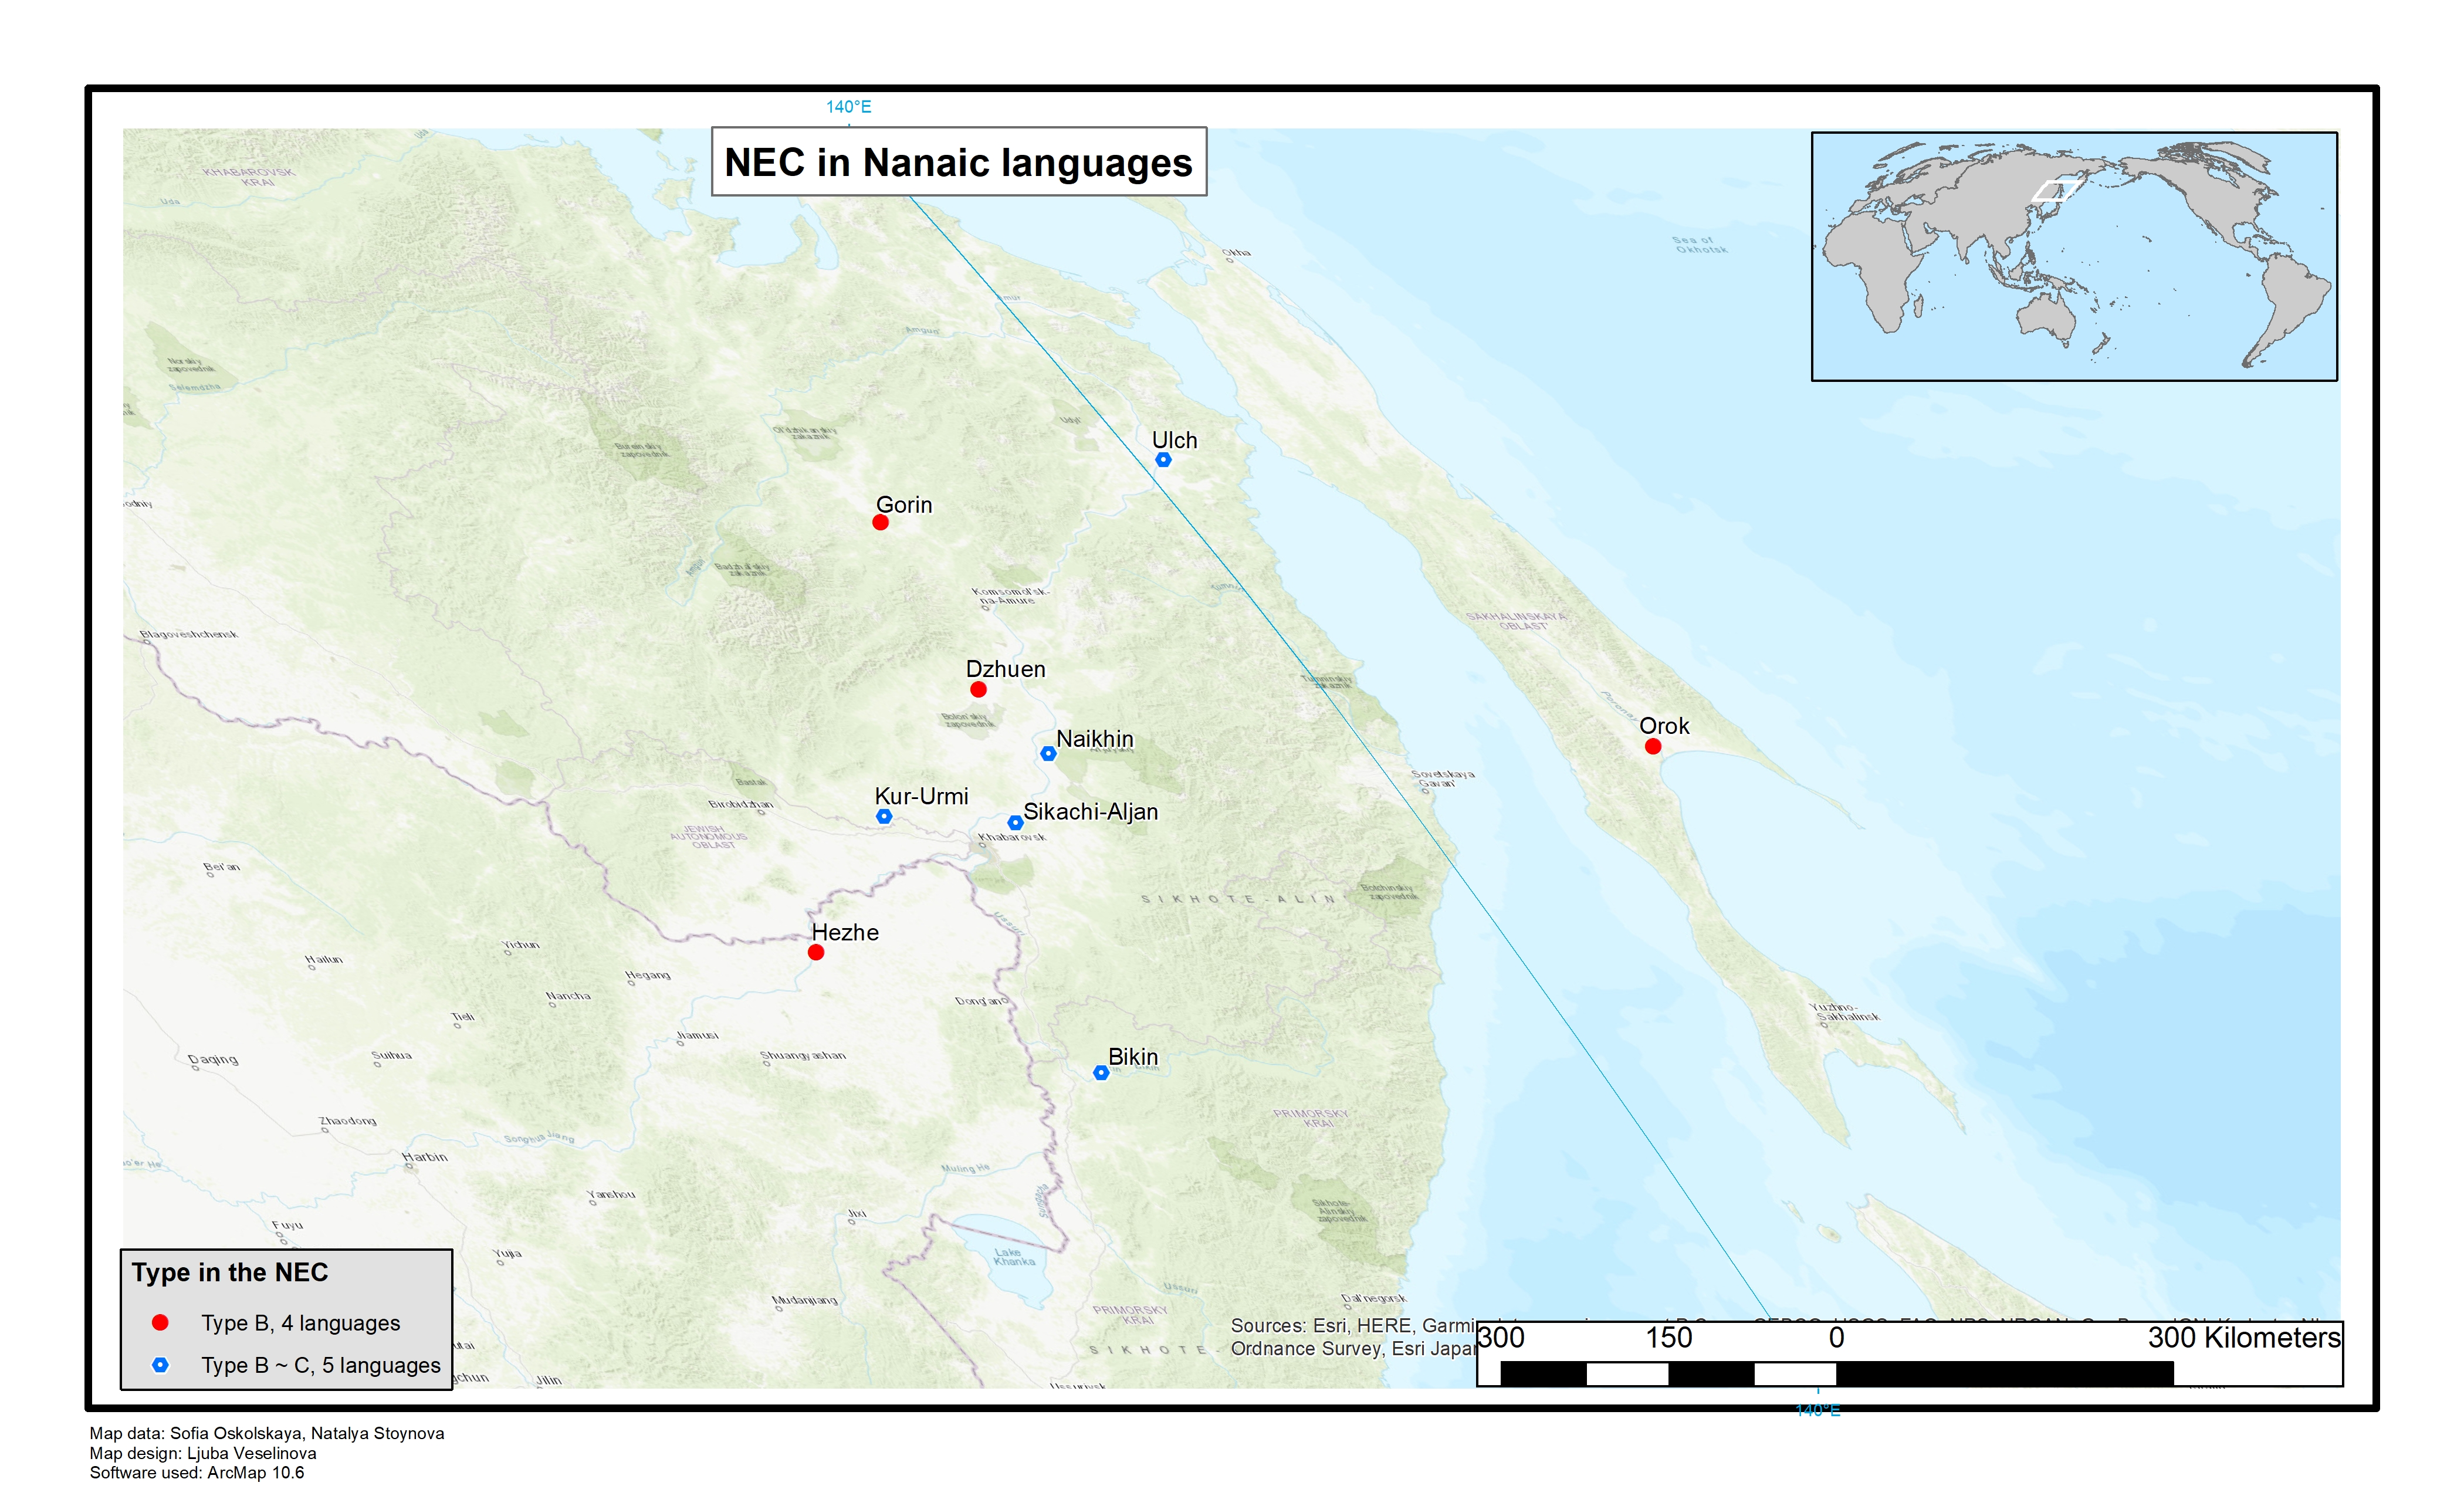
\includegraphics[width=\textwidth]{figures/NEC_in_Nanaic.jpg}
    \caption{NEC in Nanaic}
    \label{fig:NanaicMap}
\end{figure}

\begin{figure}[!h]
    \captionsetup{name=Map}
    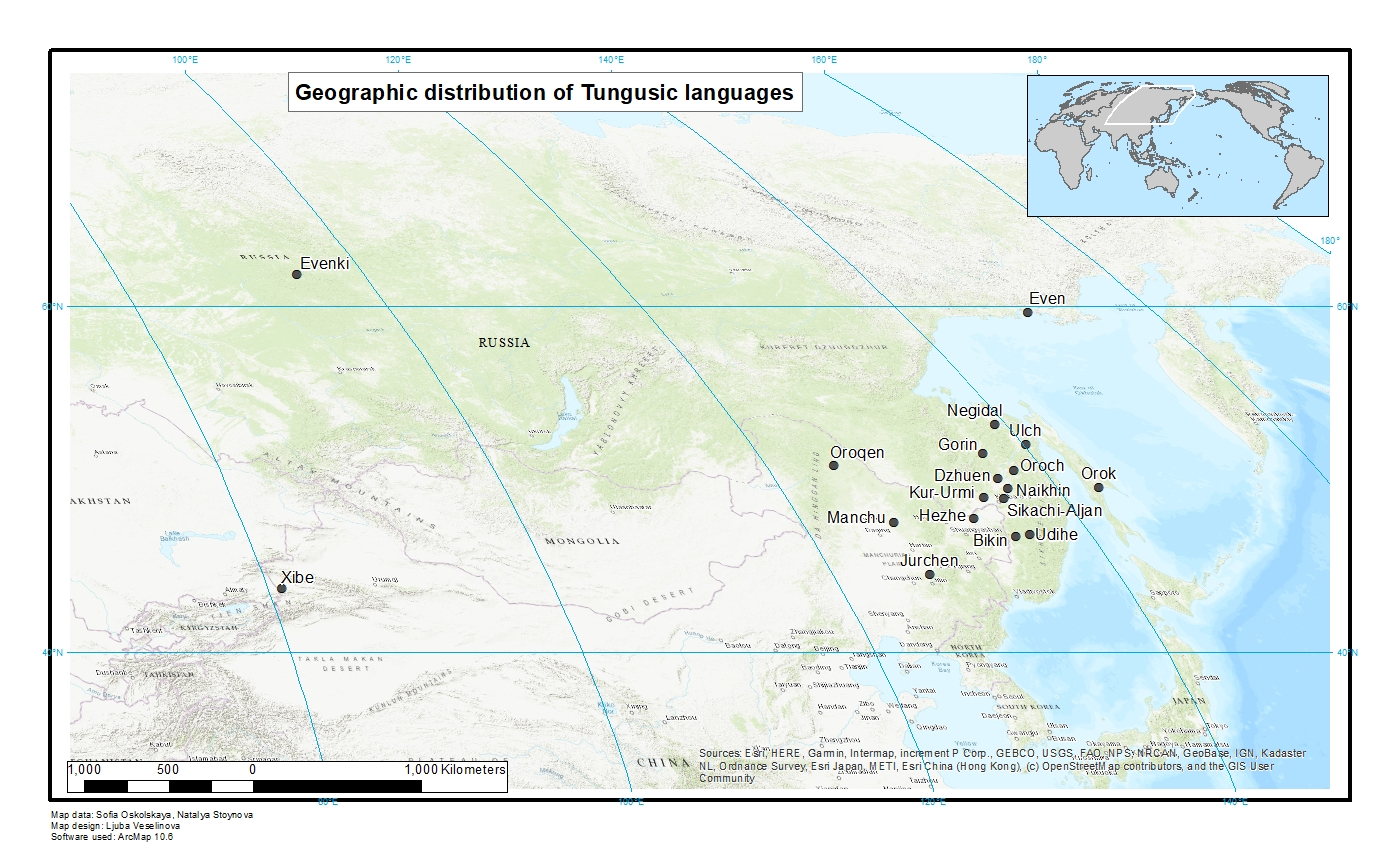
\includegraphics[width=\textwidth]{figures/Tungusic_languages.jpg}
    \caption{NEC in Tungusic}
    \label{fig:TungusicMap}
\end{figure}

\newpage

{\sloppy\printbibliography[heading=subbibliography,notkeyword=this]}



\end{document}
